\documentclass[dvipsnames, compress]{beamer}

\usepackage{currfile}
\usepackage{pgfpages}
% \setbeameroption{hide notes} % Only slides
% \setbeameroption{show only notes} % Only notes
% \setbeameroption{show notes on second screen=right} % Both
% \setbeamertemplate{note page}{\pagecolor{yellow!5}\insertnote}\usepackage{palatino}


\input{head-beamerpkg}
\usepackage{natbib}         % Pour la bibliographie
\usepackage{url}            % Pour citer les adresses web
\usepackage[T1]{fontenc}    % Encodage des accents
\usepackage[english]{babel}
\usepackage[utf8]{inputenc} % Lui aussi
\usepackage{numprint}       % Histoire que les chiffres soient bien

\usepackage{amsmath}        % La base pour les maths
\usepackage{mathtools}
\usepackage{mathrsfs}       % Quelques symboles supplémentaires
\usepackage{amssymb}        % encore des symboles.
\usepackage{amsfonts}       % Des fontes, eg pour \mathbb.
\usepackage{array}
\usepackage{cancel}
\usepackage{stackengine}    % text above other text
\usepackage{ifthen}         % ifthenelse

\usepackage{hyperref}


%%% Si jamais vous voulez changer de police: décommentez les trois
%\usepackage{tgpagella}
%\usepackage{tgadventor}
%\usepackage{inconsolata}

\usepackage{xcolor} % De la couleur
\usepackage{graphicx} % inclusion des graphiques
\usepackage{wrapfig}  % Dessins dans le texte.

\usepackage{listings} % Code blocks
\usepackage{rustlistings}

% \usepackage{tabulary} % 

\usepackage{tikz}     % Un package pour les dessins (utilisé pour l'environnement {code})
%\usepackage{tikz-cd}
\usetikzlibrary{automata,positioning,arrows,trees}
\usetikzlibrary{decorations.pathreplacing}
\usepackage{adjustbox}
\usepackage[framemethod=TikZ]{mdframed}

\usepackage{pifont} % extra symbols


% Ce fichier contient toutes les macros que vous pouvez avoir envie de définir
% si vous les utilisez plusieurs fois dans le document.

\PassOptionsToPackage{svgnames}{color}

% Un environnement pour bien présenter le code informatique
\newenvironment{code}{%
\begin{mdframed}[linecolor=green,innerrightmargin=30pt,innerleftmargin=30pt,
backgroundcolor=black!5,
skipabove=10pt,skipbelow=10pt,roundcorner=5pt,
splitbottomskip=6pt,splittopskip=12pt]
}{%
\end{mdframed}
}

\newcommand{\bijective}{%
  \hookrightarrow\mathrel{\mspace{-15mu}}\rightarrow
}
\newcommand{\surjective}{\twoheadrightarrow}
\newcommand{\injective}{\hookrightarrow}
\newcommand{\implication}{\Longrightarrow}
\newcommand{\impl}{\Rightarrow}
\newcommand{\reciprocal}{\Longleftarrow}
\newcommand{\equivalent}{\Longleftrightarrow}
\newcommand{\NN}{\ensuremath{\mathbb{N}}}
\newcommand{\RR}{\ensuremath{\mathbb{R}}}
\newcommand{\QQ}{\ensuremath{\mathbb{Q}}}
\newcommand{\ZZ}{\ensuremath{\mathbb{Z}}}
\newcommand{\CC}{\ensuremath{\mathbb{C}}}
\newcommand{\EE}{\ensuremath{\mathbb{E}}}
\newcommand{\PP}{\ensuremath{\mathbb{P}}}
\renewcommand{\epsilon}{\varepsilon}
\renewcommand{\phi}{\varphi}
\renewcommand{\leq}{\leqslant}
\renewcommand{\geq}{\geqslant}

\newcommand{\bbrack}[1]{\left\llbracket#1\right\rrbracket}

\newcommand{\inv}[1]{#1^{-1}}

\newcommand{\tsf}[1]{\textsf{#1}}
\newcommand{\ttt}[1]{\texttt{#1}}
\newcommand{\tbf}[1]{\textbf{#1}}
\newcommand{\tsc}[1]{\textsc{#1}}
\newcommand{\tq}{\ |\ }
\newcommand{\abs}[1]{\ensuremath{\left|#1\right|}}
\newcommand{\set}[1]{\ensuremath{\left\{#1\right\}}}
\newcommand{\paren}[1]{\ensuremath{\left(#1\right)}}

\newcommand\semantics{%
    \mathrel{\rightsquigarrow}}


\newlength{\mirageWidth}\newlength{\mirageHeight}
\newcommand{\mirage}[1]{% The opposite of a \phantom: it is visible but it takes no space
    #1%
    \settowidth{\mirageWidth}{#1}%
    \settoheight{\mirageHeight}{#1}%
    \hspace{-\mirageWidth}%
    \vspace{-\mirageHeight}%
}

\DeclareMathOperator{\poly}{poly}
\DeclareMathOperator{\expn}{exp}
\DeclareMathOperator{\minvolume}{\exists\textup{\tsf{MVol}}}
\DeclareMathOperator{\avgvolume}{\textup{\tsf{EMVol}}}
\DeclareMathOperator{\maxvolume}{\textup{\tsf{DMVol}}}
\DeclareMathOperator{\radius}{\textup{\tsf{MRad}}}
\newcommand{\neigh}{\mathcal{N}}

\newenvironment{stacked}{%
    \begin{tikzpicture}%
        \node (ref) {};%
}{%
    \end{tikzpicture}%
}

\newcommand{\stackitem}[2]{%
    \node at (ref) {{%
        \visible<#1>{%
            \begin{minipage}{\textwidth}
                #2%
            \end{minipage}
        }%
    }};%
}

\newcommand{\runnable}[2]{%
    \begin{block}{Demo}%
        \href{run:run/#1.sh}{\texttt{#2}}%
    \end{block}%
}


\title[TreeBor]{Tree Borrows}
\subtitle{An aliasing model for Rust}
\author{\underline{Neven \textsc{Villani}}, Ralf \textsc{Jung}, Derek \textsc{Dreyer}}
\date{ENS Paris-Saclay and MPI-SWS Saarbr\"ucken}

\renewcommand{\familydefault}{\sfdefault}
\begin{document}


% What structure do we want for the presentation ?
% In no particular order:
%[ ] - SB basics
%[X]   - quick word on 2-phase borrows
%[X]   - same interface
%[X]   - stack structure and comparison of dimensions
%[ ] - comparison with SB
%[ ]   - are the lost optimizations important ?
%[X]     - spurious writes: can't assume termination
%[ ]   - what more code can we write ?
%[ ]     - copy_nonoverlapping is a good selling point
%[X] - derivation of the tree structure
%[X]   - with things that should not change anything significant
%[X]     - `fn(&x) { x }` ~ `fn(&x) { &*x }`
%[X]     - `*_ = 1` ~ `*(&*_) = 1`
%        showing that it is basically mandatory that we only
%        distinguish between child vs self vs foreign,
%        then the lack of distinction between child and self is a choice,
%        not a necessity.
%[X]   - some freedom in when we create a new pointer:
%        it's easy to define "equivalence classes" of "this reference
%        and all its raw copies"
%[X] - necessary rules
%[X]   - noalias requirements
%[X]   - unique path of Active
%[X] - chosen rules
%[X]   - Active -> Frozen
%[X]   - everything starts Reserved
%[X]   - not writing on function entry
%[X]   for each of these show what we would lose/gain in terms of patterns/optimizations
%      if we changed them.
%[X] - how to use / a working example
%[X]   - MIRIFLAGS
%[X]   - interpretation of errors

\begin{frame}
    \titlepage
\end{frame}

\section{Introduction}

\begin{frame}[fragile,t]
    \frametitle{Why have UB?}
    \framesubtitle{A simple(r) example}

    \begin{lstlisting}[language=rust]
enum bool {
    true = 1,
    false = 0,
}
    \end{lstlisting}

    \begin{onlyenv}<2>
        What happens if...
        \begin{lstlisting}[language=rust]
let b: bool = 2;
        \end{lstlisting}
    \end{onlyenv}

    \begin{onlyenv}<3>
        What happens if...
        \begin{lstlisting}[language=rust]
let b: bool = unsafe { std::mem::transmute(2) };
//             ^^^^^^ remember this
let notb = !b; // ?
let notnotb = !notb;
assert!(b == notnotb); // ???
        \end{lstlisting}
        Can the compiler optimize a double negation into the identity ?
    \end{onlyenv}

    \begin{onlyenv}<4>
        What happens if...
        \begin{lstlisting}[language=rust, escapechar=@]
let b: bool = unsafe { std::mem::transmute(2) };
// UB: invalid value
@@
@@
@@
        \end{lstlisting}
        The compiler \textit{can} optimize a double negation into the identity.\\
        The compiler can do \textit{anything} once you have constructed an invalid value.
    \end{onlyenv}
\end{frame}

\begin{frame}[fragile]
    \frametitle{Rust's type system}
    \begin{onlyenv}<1>
        \begin{lstlisting}[language=rust]
let t: T = v;
//          ^ value
//      ^ type
//  ^ variable
//  ^^^^^^^^ variable binding

fn incr(n: u8) -> u8 {
    n + 1
}

fn main() {
    let n: u8 = 42;
    let m: u8 = incr(n);
    println!("{n} + 1 = {m}");
}
        \end{lstlisting}
    \end{onlyenv}

    \begin{onlyenv}<2>
        \begin{lstlisting}[language=rust]
// Primitives
f32, f64, u8, i8, u16, i16, u32, i32,
u64, i64, u128, i128, usize, isize, bool
// Products
struct Point {
    x: f64,
    y: f64,
}
type Triplet = (f64, f64, usize);
type Array = [f64; 10];
// Sums
enum Shape {
    Circle(Point, f64),
    Square(Point, f64),
    Triangle([Point; 3]),
}
        \end{lstlisting}
    \end{onlyenv}

    \begin{onlyenv}<3>
        \begin{lstlisting}[language=rust, escapechar=@]
// Smart pointers
Box<T>, Rc<T>, Arc<T>, Cow<T>

// Raw pointers
*const T
*mut T
// (*const T @\(\sqsubset\)@ *mut T)

// References
@@&'a T // shared and immutable
@@&'a mut T // unique and mutable
// (&'a T @\(\sqsubset\)@ &'a mut T)
// ('a @\(\subset\)@ 'b @\(\Rightarrow\)@ &'a T @\(\sqsubset\)@ &'b T)
// ('a @\(\subset\)@ 'b @\(\Rightarrow\)@ &'a mut T @\(\sqsubset\)@ &'b mut T)
        \end{lstlisting}
    \end{onlyenv}

    \begin{onlyenv}<4>
        Just like
        \begin{lstlisting}[language=rust]
// x: &mut bool
*x = 4;
        \end{lstlisting}
        is a type error (mismatched types \texttt{bool} and \texttt{u8}),
        \begin{lstlisting}[language=rust]
// x: &u8
*x = 4;
        \end{lstlisting}
        is also a type error (\texttt{\&\_} does not support assignment),
        and so is
        \begin{lstlisting}[language=rust]
// n: u8
let p = (&mut n, &mut n);
        \end{lstlisting}
        (impossible to satisfy lifetime constraints).\\

        Mutability and uniqueness are part of the type!\\
        Can we exploit that?
    \end{onlyenv}

\end{frame}

\begin{frame}[fragile,t]
    \frametitle{What is \texttt{unsafe}?}
    The type system of Rust is a bit too strict for some low-level applications.\\
    The \texttt{unsafe} keyword gives access to the language \textit{unsafe Rust},
    superset of Rust, where you can
    \begin{itemize}
        \item dereference raw pointers,
        \item call \texttt{unsafe} functions,
        \item do ffi.
    \end{itemize}

    This has the effect of making \texttt{unsafe} an escape hatch to locally bypass the type checker.
    \begin{exampleblock}{From the previous example}
        \texttt{std::mem::transmute} is an \texttt{unsafe} function, thus the
        use of \texttt{unsafe \{ std::mem::transmute(2) \}}.
    \end{exampleblock}
\end{frame}

\begin{frame}[fragile, t]
    \frametitle{A motivating example for Aliasing UB}
    \begin{lstlisting}[language=rust]
fn foo(x: &mut u64) {
    let val = *x;
    opaque();
    *x = val;
}
    \end{lstlisting}
    optimized into
    \begin{lstlisting}[language=rust]
fn foo(x: &mut u64) {
    opaque();
}
    \end{lstlisting}
    Well-typedness of any program that calls \texttt{foo} implies uniqueness
    of \texttt{x} during the execution of \texttt{foo}: \texttt{opaque} cannot mutate \texttt{x}!\\
    \begin{onlyenv}<2->
    ...except if the user uses \texttt{unsafe} to bypass the uniqueness check\\
    \end{onlyenv}
    \begin{onlyenv}<3>
    ...which we are going to assume does not happen: we will declare it to be UB
    to use \texttt{unsafe} to violate the requirement of uniqueness on mutable references.
    \end{onlyenv}
\end{frame}

\begin{frame}[t]
    \frametitle{Tree Borrows: specification and detection of pointer aliasing UB}
    \begin{alertblock}{Starting observation}
        Proper usage of pointers (lifetime inclusion and inheritance of mutability) follows a tree discipline.
    \end{alertblock}
    \begin{block}{Key ideas}
        \begin{itemize}
            \item per-location tracking of pointers
            \item use a tree to store pointer identifiers
            \item on each reborrow a new identifier is added as a leaf of the tree
            \item each pointer has permissions
            \item a pointer can be used if its permission allows it (to be defined)
            \item using a pointer makes incompatible (to be defined) pointers lose permissions
        \end{itemize}
    \end{block}
\end{frame}



\section{Tree Structure}

\begin{frame}[fragile]
    \frametitle{A Tree of pointers}
    \begin{minipage}{0.27\textwidth}
        \begin{block}{}
            \begin{tikzpicture}[
                every node/.append style = {anchor = west},
                grow via three points={one child at (0.5,-0.8) and two children at (0.5,-0.8) and (0.5,-1.6)},
                edge from parent path={(\tikzparentnode\tikzparentanchor) |- (\tikzchildnode\tikzchildanchor)}]
            \node at (0,0) {\texttt{x}}
                child {node {\texttt{y1}}
                    child {node {\texttt{y2}}}}
                child[missing] {}
                child {node {\texttt{z1}, \texttt{z2}}}
                child {node {\texttt{w1}}
                    child {node {\texttt{w2}}
                        child {node {\texttt{w3}}}}};
            \end{tikzpicture}
        \end{block}
    \end{minipage}
    ~\ ~\
    \begin{minipage}{0.65\textwidth}
        \begin{block}{}
            \begin{lstlisting}[language=rust]
let x = &mut 0u64; // initial borrow

let y1 = &mut *x; // mutable reborrow
let y2 = &*y1; // shared reborrow

let z1 = &*x;
let z2 = z1 as *const u64; // cast

foo(x); // implicit mutable reborrow
fn foo(w2: &mut u64) {
    let w3 = &*w2;
}

            \end{lstlisting}
        \end{block}
    \end{minipage}
\end{frame}

\begin{frame}
    \frametitle{What's in the tree ?}
    Each pointer is given a tag~\\~\\

    Tree Borrows tracks:
    \begin{itemize}
        \item \textbf{permission}: per tag, per location;
        \item \textbf{hierarchy} between tags;
        \item accesses are done through a tag:
            \begin{itemize}
                \item \textbf{require permissions} of the tag\\
                    (UB if the permissions are insufficient)
                \item \textbf{update permissions} of other tags\\
                    (UB if the modification is forbidden)
            \end{itemize}
    \end{itemize}
\end{frame}

\begin{frame}
    \frametitle{One pointer, \(2 \times 2\) kinds of accesses}
    \begin{block}{}
        \centering
        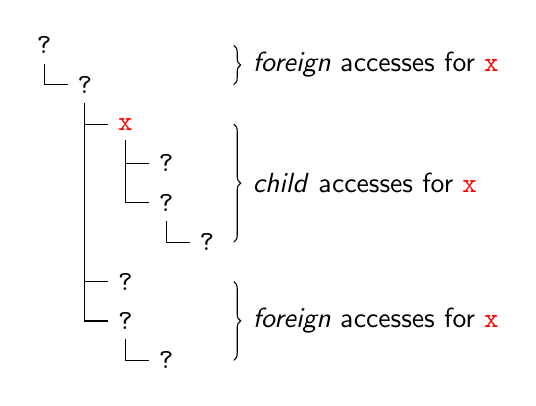
\begin{tikzpicture}[
            every node/.append style = {anchor = west},
            grow via three points={one child at (0.3,-0.5) and two children at (0.3,-0.5) and (0.3,-1.0)},
            edge from parent path={(\tikzparentnode\tikzparentanchor) |- (\tikzchildnode\tikzchildanchor)}]
            \node (root) at (0,0) {\texttt{?}}
                child {node (nfather) {\texttt{?}}
                    child {node (nxfirst) {\color{red}\texttt{x}}
                        child {node {\texttt{?}}}
                        child {node {\texttt{?}}
                            child {node (nxlast) {\texttt{?}}}}}
                    child[missing] {}
                    child[missing] {}
                    child[missing] {}
                    child {node (nnextfirst) {\texttt{?}}}
                    child {node {\texttt{?}}
                        child {node (nnextlast) {\texttt{?}}}}}
                ;
            \draw (2.5,0 |- root) node (vmark) {};
            \draw [decorate, decoration = {brace}] (vmark |- nxfirst) -- (vmark |- nxlast)
                node[midway] {~\textit{child} accesses for \color{red}\texttt{x}};
            \draw [decorate, decoration = {brace}] (vmark |- root) -- (vmark |- nfather)
                node[midway] {~\textit{foreign} accesses for \color{red}\texttt{x}};
            \draw [decorate, decoration = {brace}] (vmark |- nnextfirst) -- (vmark |- nnextlast)
                node[midway] {~\textit{foreign} accesses for \color{red}\texttt{x}};
        \end{tikzpicture}
        ~\\
        each \textit{read} or \textit{write}.
    \end{block}
\end{frame}

\begin{frame}[fragile]
    \frametitle{Kinds of accesses: examples}
    \begin{block}{}
        \begin{lstlisting}[language=rust]
let x = &mut ...;
let y = &mut *x;

*x = 1; // Write access; foreign for y; child for x.
let _ = *y; // Read access; child for y; child for x.
        \end{lstlisting}
    \end{block}
    \begin{block}{}
        \centering
        \begin{tikzpicture}[
            every node/.append style = {anchor = west},
            grow via three points={one child at (0.3,-0.5) and two children at (0.3,-0.5) and (0.3,-1.0)},
            edge from parent path={(\tikzparentnode\tikzparentanchor) |- (\tikzchildnode\tikzchildanchor)}]
            \node {...}
                child {node {\texttt{x}}
                    child {node {\texttt{y}}}};
        \end{tikzpicture}
    \end{block}
\end{frame}


\section{Deriving rules}

\begin{frame}
    \frametitle{}
\end{frame}


\section{Optimizations}

\begin{frame}
    \frametitle{Some standard optimizations}
    \newcommand{\asterisk}{\textsuperscript{*}}
    \newcommand{\noasterisk}{\phantom{\asterisk}}
    \begin{tabular}{|l|c|c|l}
        \cline{1-3}
        Possible in...                     & SB     & TB &\\
        \cline{1-3}
        Swap call-read \(\to\) read-call (speculative)
            & \cmark\noasterisk
            & \cmark\noasterisk
            &\\
        \cline{1-3}
        Swap read-call \(\to\) call-read
            & \cmark\asterisk
            & \cmark\asterisk
            &\\
        \(\triangleright\)\scriptsize~ Swap read-read' \(\to\) read'-read
            & \scriptsize \cmark\asterisk
            & \scriptsize \cmark\noasterisk
            & \visible<3>{\(\gets\) TB only}\\
        \cline{1-3}
        Swap call-write \(\to\) write-call (speculative)
            & \cmark\asterisk
            & \xmark\noasterisk
            & \visible<2>{\(\gets\) SB only}\\
        \(\triangleright\)\scriptsize~ Swap write-call-write \(\to\) write-write-call
            & \scriptsize \cmark\asterisk
            & \scriptsize \cmark\asterisk
            &\\
        \cline{1-3}
        Swap write-call \(\to\) call-write
            & \cmark\asterisk
            & \cmark\asterisk
            &\\
        \(\triangleright\)\scriptsize~ Swap write-read'-read \(\to\) read'-write-read
            & \scriptsize \cmark\noasterisk
            & \scriptsize \cmark\asterisk
            & \visible<2>{\(\gets\) SB only}\\
        \cline{1-3}
    \end{tabular}~\\~\\

    {\footnotesize
    all are possible for references without interior mutability\\
    (\texttt{\&mut} if a write is involved, both \texttt{\&} and \texttt{\&mut} if read-only)\\
    \asterisk: only for protected references\\
    }
\end{frame}

\subsection{Possible optimizations}

\newcommand{\assumepath}[2]{\textover{\visible<#1>{\color{magenta}{#2}}}{}}

\begin{frame}[fragile, t]
    \frametitle{Swap write-write}

    \begin{onlyenv}<1-3>
        \begin{block}{{\cmark} Base model}
            \begin{lstlisting}[language=rust, escapechar=@]
let x = &mut ...;
let y = &mut ...;
*x = 42; // (optimization: move down ?)
*y = 19; // is this a foreign write ? @\assumepath{2}{if not}\assumepath{3}{if yes}@

*x = 57;
            \end{lstlisting}
        \end{block}%
        \includegraphics<1>{blank.base.pdf}%
        \includegraphics<2>{path.base.mut+cw+cw.pdf}%
        \includegraphics<3>{path.base.mut+cw+fw+cw.pdf}%
    \end{onlyenv}

    \begin{onlyenv}<4>
        \begin{block}{{\cmark} Base model}
            \begin{lstlisting}[language=rust, escapechar=@]
let x = &mut ...;
let y = &mut ...;

*y = 19; // assumed not to be a foreign write
*x = 42;
*x = 57;
            \end{lstlisting}
        \end{block}
        \includegraphics{path.base.mut+cw+cw.pdf}
    \end{onlyenv}

    \begin{onlyenv}<5>
        \begin{block}{{\cmark} Base model}
            \begin{lstlisting}[language=rust, escapechar=@]
let x = &mut ...;
let y = &mut ...;

*y = 19; // assumed not to be a foreign write

*x = 57;
            \end{lstlisting}
        \end{block}
        \includegraphics{path.base.mut+cw.pdf}
    \end{onlyenv}
\end{frame}

\begin{frame}[fragile, t]
    \frametitle{Insert speculative read}
    \begin{onlyenv}<1-4>
        \begin{block}{{\cmark} Base model}
            \begin{lstlisting}[language=rust, escapechar=@]
fn read(x: &u64) -> u64 {

    opaque(/* contains foreign access ? @\assumepath{2}{if none}\assumepath{3}{if read}\assumepath{4}{if write}\phantom{........}@ */);
    *x // (optimization: move up ?)
}
            \end{lstlisting}
        \end{block}
        \includegraphics<1>{blank.base.pdf}
        \includegraphics<2>{path.prot.shr+cr.pdf}
        \includegraphics<3>{path.prot.shr+cr+fr.pdf}
        \includegraphics<4>{path.prot.shr+fw.pdf}
    \end{onlyenv}

    \begin{onlyenv}<5>
        \begin{block}{{\cmark} Base model}
            \begin{lstlisting}[language=rust, escapechar=@]
fn read(x: &u64) -> u64 {
    let val = *x;
    opaque(/* assume no foreign write */);
    val
}
            \end{lstlisting}
        \end{block}
        \includegraphics{path.prot.shr+cr+fr.pdf}
    \end{onlyenv}
\end{frame}

\subsection{Impossible optimizations}

\begin{frame}[fragile, t]
    \frametitle{Insert speculative write}

    \begin{block}{{\xmark} Base model}
        \begin{lstlisting}[language=rust, escapechar=@]
fn foo(x: &mut u64) {

    opaque(/* contains foreign access ? @\assumepath{2}{if write}\assumepath{3}{if read}\assumepath{4}{if read+loop}\phantom{............}@ */);
    *x = 42; // (optimization: move up ?)
}
        \end{lstlisting}
    \end{block}
    \includegraphics<1>{blank.base.pdf}
    \includegraphics<2>{path.prot.mut+fw.pdf}
    \includegraphics<3>{path.prot.mut+fr+cw.pdf}
    \includegraphics<4>{path.prot.mut+fr.pdf}
\end{frame}

\begin{frame}[fragile]
    \frametitle{Insert speculative write: strengthening}
    \begin{onlyenv}<1-2>
        \begin{exampleblock}{Possible strengthening}
            Write to mutable references of function entry
        \end{exampleblock}
        \includegraphics<1>[width=0.7\textwidth]{mod.full.pdf}
        \includegraphics<2>[width=0.7\textwidth]{steps.prot+w.pdf}
    \end{onlyenv}

    \begin{onlyenv}<3-4>
        \begin{block}{{\cmark} Strengthened model}
            \begin{lstlisting}[language=rust, escapechar=@]
fn foo(x: &mut u64) {

    opaque(/* contains foreign access ? @\assumepath{3}{if none}\assumepath{4}{if any}\phantom{.......}@ */);
    *x = 42;
}
            \end{lstlisting}
        \end{block}
        \includegraphics<3>{path.prot+w.mut.pdf}
        \includegraphics<4>{path.prot+w.mut+fr-fw.pdf}
    \end{onlyenv}

    \begin{onlyenv}<5>
        \begin{block}{{\cmark} Strengthened model}
            \begin{lstlisting}[language=rust, escapechar=@]
fn foo(x: &mut u64) {
    *x = 42;
    opaque(/* assume no foreign access */);

}
            \end{lstlisting}
        \end{block}
        \includegraphics<5>{path.prot+w.mut+cw.pdf}
    \end{onlyenv}
\end{frame}

\begin{frame}[fragile, t]
    \frametitle{Insert speculative write: blocker}

    \begin{exampleblock}{\texttt{as\_mut\_ptr}: \textover{\visible<1-3>{base model}}{}\textover{\visible<4-5>{strengthened}}{}}
        \begin{itemize}
            \item \texttt{\&mut [T] -> *mut T}
            \item returns \textover{\visible<1-3>{a \texttt{Reserved}}}{}\textover{\visible<4-5>{an \texttt{Active}}}{}\phantom{aaaaaaaaaa.} child of the input
        \end{itemize}
    \end{exampleblock}

    \begin{block}{\textover{\visible<1-3>{\cmark}}{}\textover{\visible<4-5>{\xmark}}{}\phantom{\xmark} Common pattern}
        \begin{lstlisting}[language=rust, basicstyle=\ttfamily\scriptsize]
let raw = buf.as_mut_ptr();
let shr = buf.as_ptr().add(1);
copy_nonoverlapping(shr, raw, 1);
        \end{lstlisting}
    \end{block}

    \begin{onlyenv}<1-3>
        \begin{onlyenv}<1>
            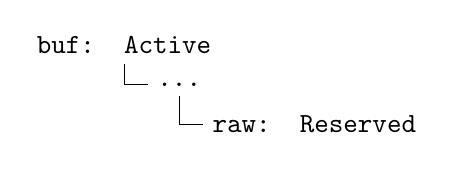
\begin{tikzpicture}[
                every node/.append style = {anchor = west},
                grow via three points={one child at (0.3,-0.5) and two children at (0.3,-0.5) and (0.3,-1.0)},
                edge from parent path={(\tikzparentnode\tikzparentanchor) |- (\tikzchildnode\tikzchildanchor)}
                ]
                \node[anchor=west] (nbuf) at (0,0) {\texttt{buf:\textover{ Active}{}}}
                        child {node {\texttt{...}}
                            child {node (nraw) {\texttt{raw: Reserved}}}}
                        ;
            \end{tikzpicture}
        \end{onlyenv}
        \begin{onlyenv}<2>
            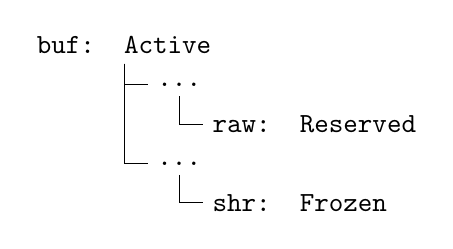
\begin{tikzpicture}[
                every node/.append style = {anchor = west},
                grow via three points={one child at (0.3,-0.5) and two children at (0.3,-0.5) and (0.3,-1.0)},
                edge from parent path={(\tikzparentnode\tikzparentanchor) |- (\tikzchildnode\tikzchildanchor)}
                ]
                \node[anchor=west] (nbuf) at (0,0) {\texttt{buf:\textover{ Active}{}}}
                        child {node {\texttt{...}}
                            child {node (nraw) {\texttt{raw: Reserved}}}}
                        child[missing] {}
                        child {node {\texttt{...}}
                            child {node (nshr) {\texttt{shr: Frozen}}}}
                        ;
            \end{tikzpicture}
        \end{onlyenv}
        \begin{onlyenv}<3>
            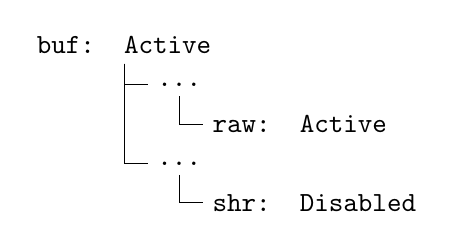
\begin{tikzpicture}[
                every node/.append style = {anchor = west},
                grow via three points={one child at (0.3,-0.5) and two children at (0.3,-0.5) and (0.3,-1.0)},
                edge from parent path={(\tikzparentnode\tikzparentanchor) |- (\tikzchildnode\tikzchildanchor)}
                ]
                \node[anchor=west] (nbuf) at (0,0) {\texttt{buf:\textover{ Active}{}}}
                        child {node {\texttt{...}}
                            child {node (nraw) {\texttt{raw: Active}}}}
                        child[missing] {}
                        child {node {\texttt{...}}
                            child {node (nshr) {\texttt{shr: Disabled}}}}
                        ;
            \end{tikzpicture}
        \end{onlyenv}

    \end{onlyenv}

    \begin{onlyenv}<4-5>
        \begin{onlyenv}<4>
            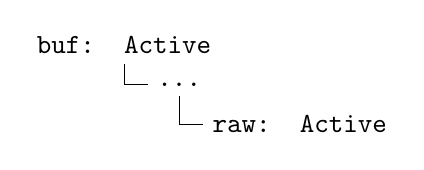
\begin{tikzpicture}[
                every node/.append style = {anchor = west},
                grow via three points={one child at (0.3,-0.5) and two children at (0.3,-0.5) and (0.3,-1.0)},
                edge from parent path={(\tikzparentnode\tikzparentanchor) |- (\tikzchildnode\tikzchildanchor)}
                ]
                \node[anchor=west] (nbuf) at (0,0) {\texttt{buf:\textover{ Active}{}}}
                        child {node {\texttt{...}}
                            child {node (nraw) {\texttt{raw: Active}}}}
                        ;
            \end{tikzpicture}
        \end{onlyenv}
        \begin{onlyenv}<5>
            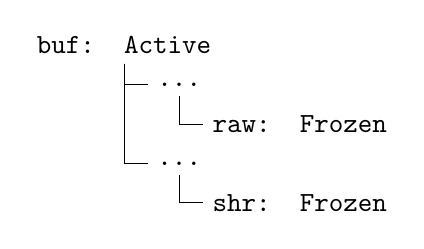
\begin{tikzpicture}[
                every node/.append style = {anchor = west},
                grow via three points={one child at (0.3,-0.5) and two children at (0.3,-0.5) and (0.3,-1.0)},
                edge from parent path={(\tikzparentnode\tikzparentanchor) |- (\tikzchildnode\tikzchildanchor)}
                ]
                \node[anchor=west] (nbuf) at (0,0) {\texttt{buf:\textover{ Active}{}}}
                        child {node {\texttt{...}}
                            child {node (nraw) {\texttt{raw: Frozen}}}}
                        child[missing] {}
                        child {node {\texttt{...}}
                            child {node (nshr) {\texttt{shr: Frozen}}}}
                        ;
            \end{tikzpicture}
        \end{onlyenv}
    \end{onlyenv}
\end{frame}

\begin{frame}[fragile, t]
    \frametitle{Swap write-read'-read \(\to\) read'-write-read}
    \begin{block}{{\xmark} Base model}
        \begin{lstlisting}[language=rust, escapechar=@]
let x = &mut ...;
*x = 42; // (optimization: move down ?)
let y = &...;
let vy = *y; // is this read foreign ? @\assumepath{1}{maybe}@

let vx = *x;
        \end{lstlisting}
    \end{block}
    \includegraphics{path.base.mut+cw+fr-o+cr.pdf}
\end{frame}

\begin{frame}[fragile, t]
    \frametitle{Swap write-read'-read \(\to\) write-read-read': strengthening}
    \begin{onlyenv}<1-2>
        \begin{exampleblock}{Possible strengthening}
            Foreign read makes \texttt{Active} become \texttt{Disabled}
            (rather than \texttt{Frozen})
        \end{exampleblock}
        \includegraphics<1>{mod.base.pdf}
        \includegraphics<2>{steps.base+d.pdf}
    \end{onlyenv}

    \begin{onlyenv}<3-4>
        \begin{block}{{\cmark} Strengthened model}
            \begin{lstlisting}[language=rust, escapechar=@]
let x = &mut ...;
*x = 42; // (optimization: move down ?)
let y = &...;
let vy = *y; // is this read foreign ? @\assumepath{3}{if not}\assumepath{4}{if yes}@

let vx = *x;
            \end{lstlisting}
        \end{block}
        \includegraphics<3>{path.base+d.mut+cw+cr.pdf}
        \includegraphics<4>{path.base+d.mut+cw+fr+cr.pdf}
    \end{onlyenv}

    \begin{onlyenv}<5>
        \begin{block}{{\cmark} Strengthened model}
            \begin{lstlisting}[language=rust, escapechar=@]
let x = &mut ...;

let y = &...;
let vy = *y; // read assumed not foreign
*x = 42;
let vx = *x;
            \end{lstlisting}
        \end{block}
        \includegraphics{path.base+d.mut+cw+cr.pdf}
    \end{onlyenv}
\end{frame}

\begin{frame}[fragile, t]
    \frametitle{Swap write-read'-read \(\to\) write-read-read': blocker}
    \begin{onlyenv}<1>
        \begin{block}{{\cmark} Swap read-read\vphantom{gh}}
            \begin{lstlisting}[language=rust, escapechar=@]
let y = &mut *x;
*y = 42;
let vy = *y; // (optimization: move down ?)
let vx = *x; // foreign read
@@
            \end{lstlisting}
        \end{block}
        \includegraphics{path.base.mut+cw+cr+fr.pdf}
    \end{onlyenv}

    \begin{onlyenv}<2>
        \begin{block}{{\cmark} Swap read-read\vphantom{gh}}
            \begin{lstlisting}[language=rust, escapechar=@]
let y = &mut *x;
*y = 42;

let vx = *x; // foreign read
let vy = *y;
            \end{lstlisting}
        \end{block}
        \includegraphics{path.base.mut+cw+fr+cr.pdf}
    \end{onlyenv}

    \begin{onlyenv}<3>
        \begin{block}{{\xmark} Swap read-read: strengthened model}
            \begin{lstlisting}[language=rust, escapechar=@]
let y = &mut *x;
*y = 42;
let vy = *y; // (optimization: move down ?)
let vx = *x; // foreign read
@@
            \end{lstlisting}
        \end{block}
        \includegraphics{path.base+d.mut+cw+cr+fr.pdf}
    \end{onlyenv}

    \begin{onlyenv}<4>
        \begin{block}{{\xmark} Swap read-read: strengthened model}
            \begin{lstlisting}[language=rust, escapechar=@]
let y = &mut *x;
*y = 42;

let vx = *x; // foreign read
let vy = *y;
            \end{lstlisting}
        \end{block}
        \includegraphics{path.base+d.mut+cw+fr+cr.pdf}
    \end{onlyenv}
\end{frame}

\begin{frame}
    \frametitle{Summary}
    \begin{itemize}
        \item TB allows read reorderings (SB does not)
        \item TB allows speculative reads (SB as well)
        \item TB forbids speculative writes (SB allows them)
            \begin{itemize}
                \item the model can be strengthened to justify these optimizations...
                \item ...at the cost of common patterns.
            \end{itemize}
    \end{itemize}
\end{frame}


\section{Evaluation}

\begin{frame}
    \frametitle{Counting crates with UB}
    \begin{figure}
        {\footnotesize Data obtained with the help of Ben Kimock using
        \href{https://github.com/saethlin/miri-tools}{github:saethlin/miri-tools}}
        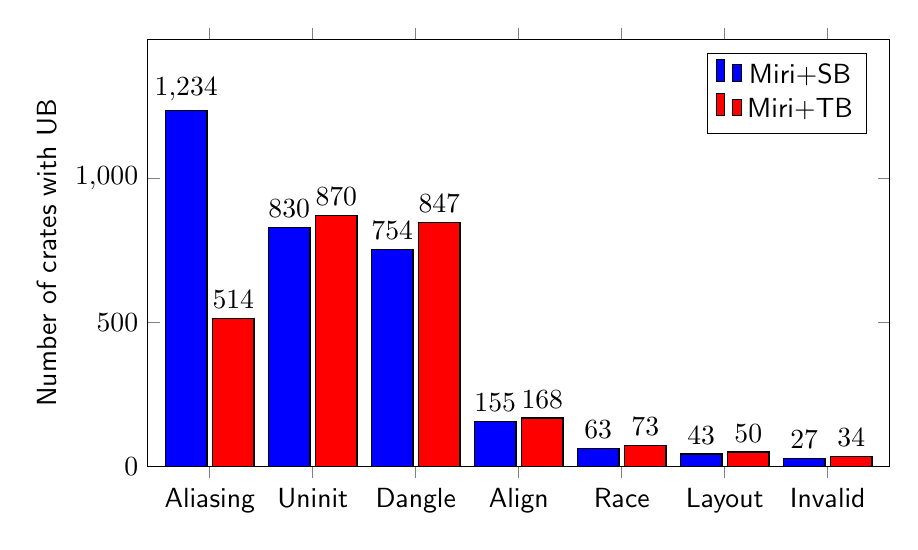
\begin{tikzpicture}
            \begin{axis}[
                    ybar,
                    ymin=0,
                    width=11cm,
                    height=7cm,
                    bar width=15pt,
                    ylabel={Number of crates with UB},
                    nodes near coords,
             %      nodes near coords align=below, % places labels inside bars
                    symbolic x coords={Aliasing, Uninit, Dangle, Align, Race, Layout, Invalid},
                    xtick = data,
                    enlarge y limits={value=0.2,upper},
                    legend pos=north east
                ]
                \addplot[fill=blue] coordinates {(Aliasing, 1234) (Uninit, 830) (Dangle, 754) (Align, 155) (Race, 63) (Layout, 43) (Invalid, 27)};
                \addplot[fill=red] coordinates {(Aliasing, 514) (Uninit, 870) (Dangle, 847) (Align, 168) (Race, 73) (Layout, 50) (Invalid, 34)};
                \legend{Miri+SB,Miri+TB}
            \end{axis}
        \end{tikzpicture}
    \end{figure}
\end{frame}

\begin{frame}
    \frametitle{Summary}
    \begin{itemize}
        \item Tree Borrows UB is much less common on \texttt{crates.io} than Stacked Borrows UB\\
            \(\qquad\Rightarrow\) fulfills goal of being more permissive
            \begin{block}{Notable examples}
                \texttt{tokio}, \texttt{pyo3}, \texttt{rkyv}, \texttt{eyre}, \texttt{ndarray},
                \texttt{arrayvec}, \texttt{slotmap}, \texttt{nalgebra}, \texttt{json}.
            \end{block}
        \item patterns allowed by Stacked Borrows but forbidden by Tree Borrows are theoretically
            possible but have not been found in actual code
    \end{itemize}
\end{frame}

\begin{frame}
    \frametitle{Reception}
    TB has existed for one year
    \begin{itemize}
        \item[$\oplus$] consensus that TB is simpler and more predictable than SB,
        \item[$\oplus$] cases where TB is more permissive than SB are welcome \\ (e.g. \texttt{\&Header} pattern),
        \item[$\oplus$] cases where TB is less permissive are rare \\ (no complaints yet),
        \item[$\ominus$] fewer optimizations (expected),
        \item[$\ominus$] controversial granularity of interior mutability,
        \item[$\ominus$] slight performance regression in Miri.
    \end{itemize}
\end{frame}

\begin{frame}
    \frametitle{Questions ?}

    TB also has...
    \begin{itemize}
        \item tweaked rules for interactions between interior mutability and protectors/\texttt{Reserved}
        \item performance improvements compared to the naive implementation
            \begin{itemize}
                \item many tricks to trim tree traversals
                \item lazy initialization for out-of-range accesses
            \end{itemize}
        \item ongoing attempt at formalization in Coq
    \end{itemize}~\\
    \vfill

    Don't hesitate to test your code with Miri and send us your interesting/unexpected cases of UB!\\~\\
    \vfill

    \href{https://github.com/Vanille-N/tree-beamer/tree/lmf}{\texttt{github:Vanille-N/tree-beamer/tree/lmf}}\\
    Complementary material: \href{https://perso.crans.org/vanille/treebor}{\texttt{perso.crans.org/vanille/treebor}}\\
\end{frame}


\end{document}
